\begin{figure}[p]
\centering
\captionsetup{justification=raggedright,labelsep=none,singlelinecheck=false,labelformat=boldlabel}
\caption[]{\footnotesize \textbf{: Gross and net Sharpe ratios for factor aggregates and multifactor allocations.} Panel A reports the long sample and Panel B the short sample. Pale bars are gross and solid bars are net of modeled factor-exposure costs. EW denotes the forecast ensemble. Each construction retains its stated exposure cap. MM and 50/50 combinations equal-weight the 153 nonmarket factors. Multifactor allocations include the market. In CMV, Random walk denotes the lagged-market signal. FCMV comparisons use HAR, HARX and the ensemble. Unmanaged denotes the matching UMV in multifactor panels.}
\label{fig:rv-portfolio_wealth_factor_panel}
\par\smallskip\textbf{Panel A. Long sample}\par\smallskip
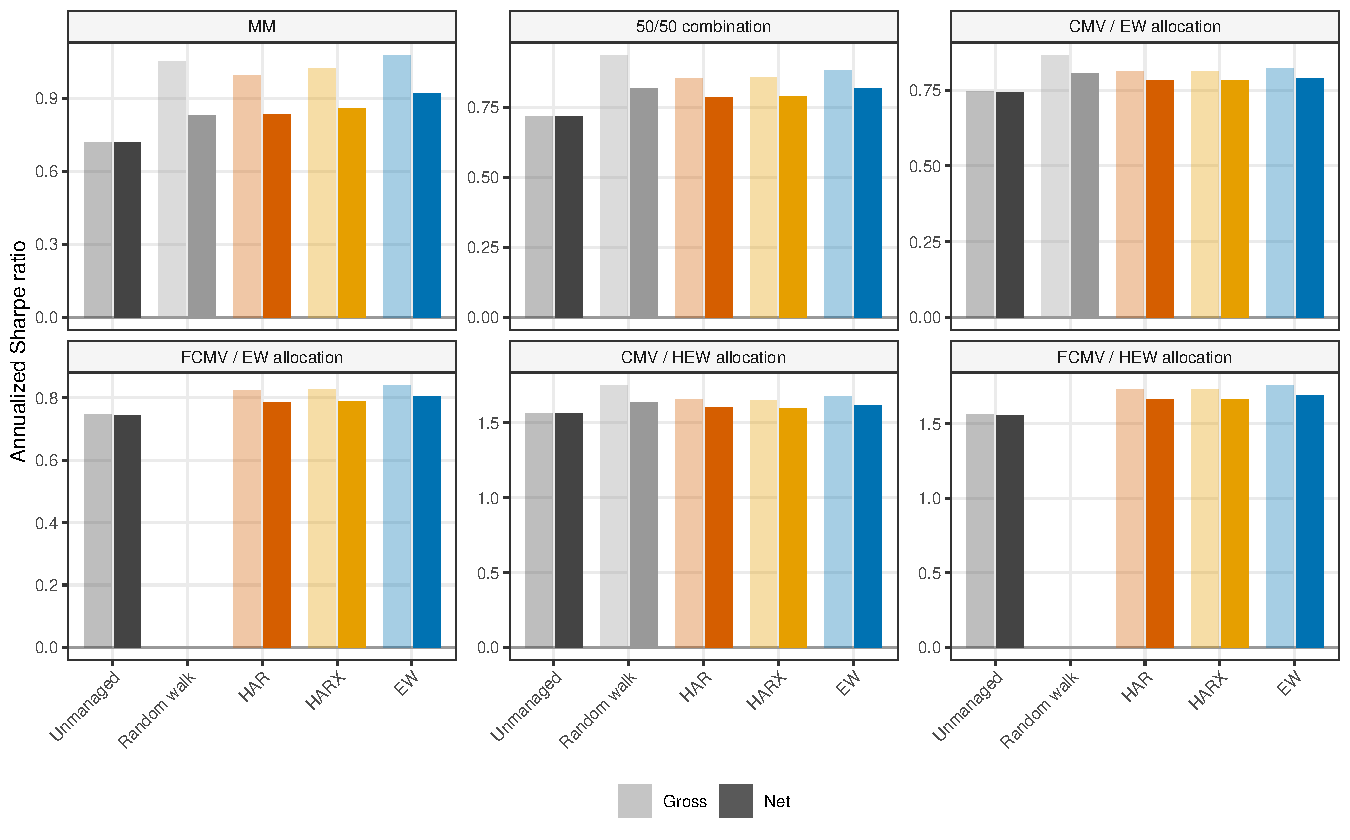
\includegraphics[width=\linewidth,height=0.70\textheight,keepaspectratio]{results_v3/combined/main_appendix/portfolio_wealth_factor_panel_1.pdf}
\end{figure}
\begin{figure}[p]
\ContinuedFloat
\centering
\captionsetup{justification=raggedright,labelsep=none,singlelinecheck=false,labelformat=boldlabel}
\caption[]{\footnotesize \textbf{: Gross and net Sharpe ratios for factor aggregates and multifactor allocations.} Panel A reports the long sample and Panel B the short sample. Pale bars are gross and solid bars are net of modeled factor-exposure costs. EW denotes the forecast ensemble. Each construction retains its stated exposure cap. MM and 50/50 combinations equal-weight the 153 nonmarket factors. Multifactor allocations include the market. In CMV, Random walk denotes the lagged-market signal. FCMV comparisons use HAR, HARX and the ensemble. Unmanaged denotes the matching UMV in multifactor panels. Continued.}
\par\smallskip\textbf{Panel B. Short sample}\par\smallskip
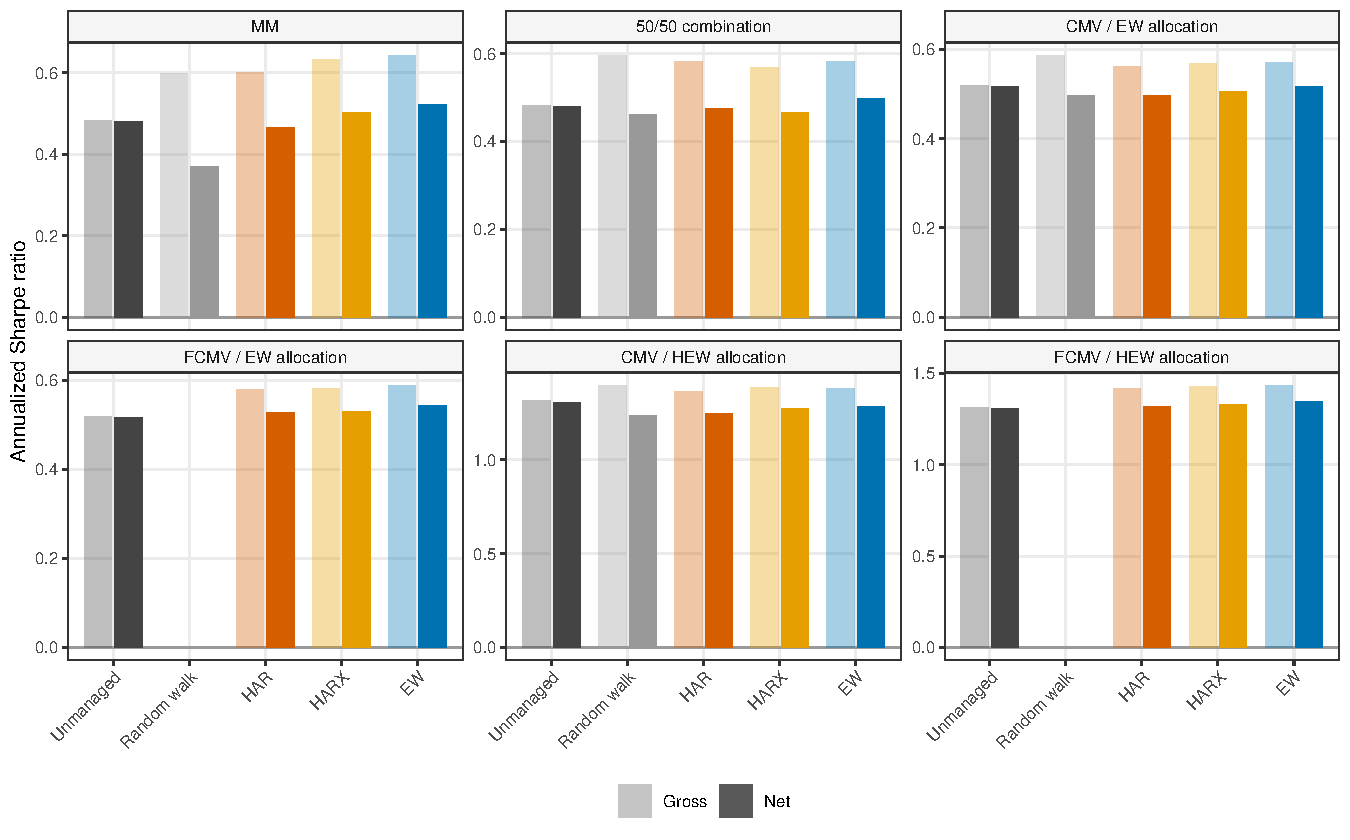
\includegraphics[width=\linewidth,height=0.70\textheight,keepaspectratio]{results_v3/combined/main_appendix/portfolio_wealth_factor_panel_2.pdf}
\end{figure}
